%!TEX root = ../final_report.tex

% \subsubsection{Building the proposal point cloud}
% \label{sssec:building_proposal_point_cloud}

% The 2D object proposals are next projected into 3D.
% For each pixel which is part of the 2D proposal, we use the known geometry of the camera to project a ray from the Kinect's optical centre through the centre of the pixel and out into the world.
% The value from the corresponding pixel in the Kinect's rectified depth map tells us how far along this ray the nearest surface is, thus giving us a point in 3D space which lies on the surface of our object candidate.

\subsubsection{Clustering the point cloud}

An issue which we discovered during the implementation phase was that the projection just described in \ref{sssec:building_proposal_point_cloud} has a certain amount of error.
Because of this error, the pixels on the outer edge of the 2D candidate would often be projected not onto the object surface but past it, meaning points on the wall or floor beyond the object would be included in the candidate point cloud (see figure \ref{fig:rays}). 

\begin{figure}[h!]
	\begin{center}
		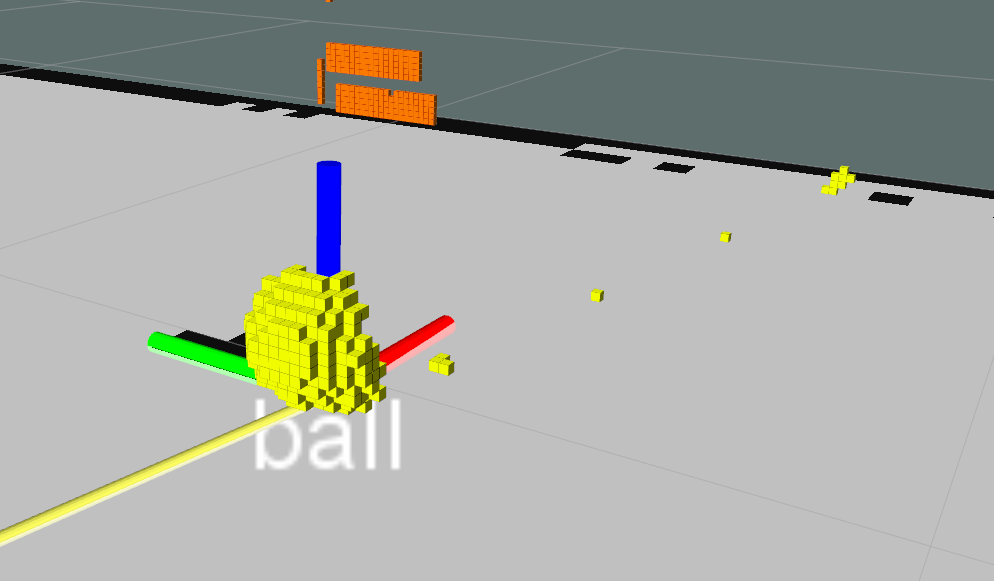
\includegraphics[width=0.5\textwidth]{src/rays2.png}
		\caption{Large parts of the ball are correctly identified; however, some additional voxels at the right side behind the ball are mistaken as belonging to the object.}
		\label{fig:rays}
	\end{center}
\end{figure}

We first attempted to overcome this difficulty by simply eroding the outermost ring of pixels from the 2D candidate before performing the projection.
However, we found that this only reduced the problem rather than solving it completely, and eroding more than a single ring of pixels from the 2D candidate resulted in an unacceptably large reduction of the candidate.

In our final system, we project the entire 2D candidate and then run PCL's Euclidean cluster extraction algorithm on the resulting point cloud.
This algorithm iteratively clusters together points which are closer to each other than a user-defined threshold, in our case \SI{2}{\centi\meter}.
We then take the cluster closest to the camera which has at least \num{50} points as our 3D proposal, which removes the outliers behind the object.

\subsubsection{Integration of point cloud into map}
\label{sssec:point_cloud_into_octomap}

The final step in our pipeline is to convert the candidate point cloud into a volumetric representation and integrate it into our octree-based 3D map.
% The 3D mapping is handled by the ROS packages \texttt{octomap_mapping}\footnote{\url{http://wiki.ros.org/octomap_mapping}} and \texttt{octomap_server}\footnote{\url{http://wiki.ros.org/octomap_server}}.
The octree itself is managed by the OctoMap framework\cite{hornung13octomap}, with ROS integration provided by the ROS package \texttt{octomap}\footnote{\url{http://wiki.ros.org/octomap}}.
Off the shelf, the \texttt{octomap} package allows for the incremental creation of a 3D occupancy grid map from point cloud data; our system extends this package to store not just occupancy information but also object candidate labels and certainty information at each node.
The certainty information stored is simply the number of times we have detected an object at that voxel and assigned it to the same object candidate label.
% \todo{Does this need more detail?}

% \subsubsection{Merging and handling of candidates in octomap}

For each point in the point cloud, \texttt{octomap} calculates into which voxel the point falls, giving a set of voxels occupied by the incoming candidate.
This set of voxels is then compared to the data in the octree to see whether we already have a belief regarding objects at that location.
If at least \SI{95}{\percent}\footnote{Setting the threshold at this level follows \cite{garcia2013computational}.} of the voxels in the incoming candidate are currently free in the octomap, then we assume that the incoming candidate is a previously unseen object.
The voxels in the candidate set are then updated as follows:
\begin{itemize}
	\item If the voxel is currently unlabelled, it is assigned the label of the incoming candidate and a certainty of \num{1}.
	\item If the voxel is currently labelled, its certainty is reduced by \num{1}. If this results in a certainty of zero, then it is assigned the incoming candidate label with a certainty of \num{1}.
\end{itemize}

If more than \SI{5}{\percent} of the voxels in the incoming candidate are already labelled in the octomap, then we assume that the candidate is part of an object which we have already seen.
The system calculates which existing object candidate the incoming candidate has the greatest overlap with and updates the voxels in the candidate set as follows:
\begin{itemize}
	\item If the voxel is currently unlabelled, it is assigned the label of the greatest overlap candidate and a certainty of \num{1}.
	\item If the voxel already has the label of the greatest overlap candidate, its certainty is increased by \num{1}.
	\item If the voxel has a different label to the greatest overlap label, its certainty is reduced by \num{1}. If this results in a certainty of zero, then it is assigned the greatest overlap label with a certainty of \num{1}.
\end{itemize}
